\chapter{Lateral Control}

\section{Exercise 1 - lateral control}
\textbf{Q. Optimize the clothoid-based lateral controller}

The clothoid-based lateral controller uses Equation \ref{eq:6.1} to calculate the steering angle required to follow the clothid. The under-steering gradient $\kus$ was calculated previously using the handling diagram and the results were shown in Table \ref{tab:6.1} and Figure \ref{64d1}. These results were implemented as a variable that changes based on the vehicle's current speed.

\begin{equation}\label{eq:6.1}
\delta(s) = k(s) (L + \kus u^2)
\end{equation}

To optimize the clothoid-based lateral controller look ahead variable, several tests were conducted using the following variables totalling 42 tests in total:

\begin{itemize}
    \item $u$ = [10, 20, 30, 40, 50, 60, 70, 80] km/h
    \item look ahead = [5, 10, 15, 20, 25, 30]
\end{itemize}

The tracking error had to be calculated to compare the tests' results. That was done by using the ``N-D nearest point search" function in Matlab, which returns indices of closest points in the desired path for each point on the real path. Then calculating the euclidean distance between each point in the real path and closest point on the desired path as tracking error. The results are shown in Figure \ref {64d1} and Table \ref{tab:6.1}.
        
        \begin{figure}[ht]
        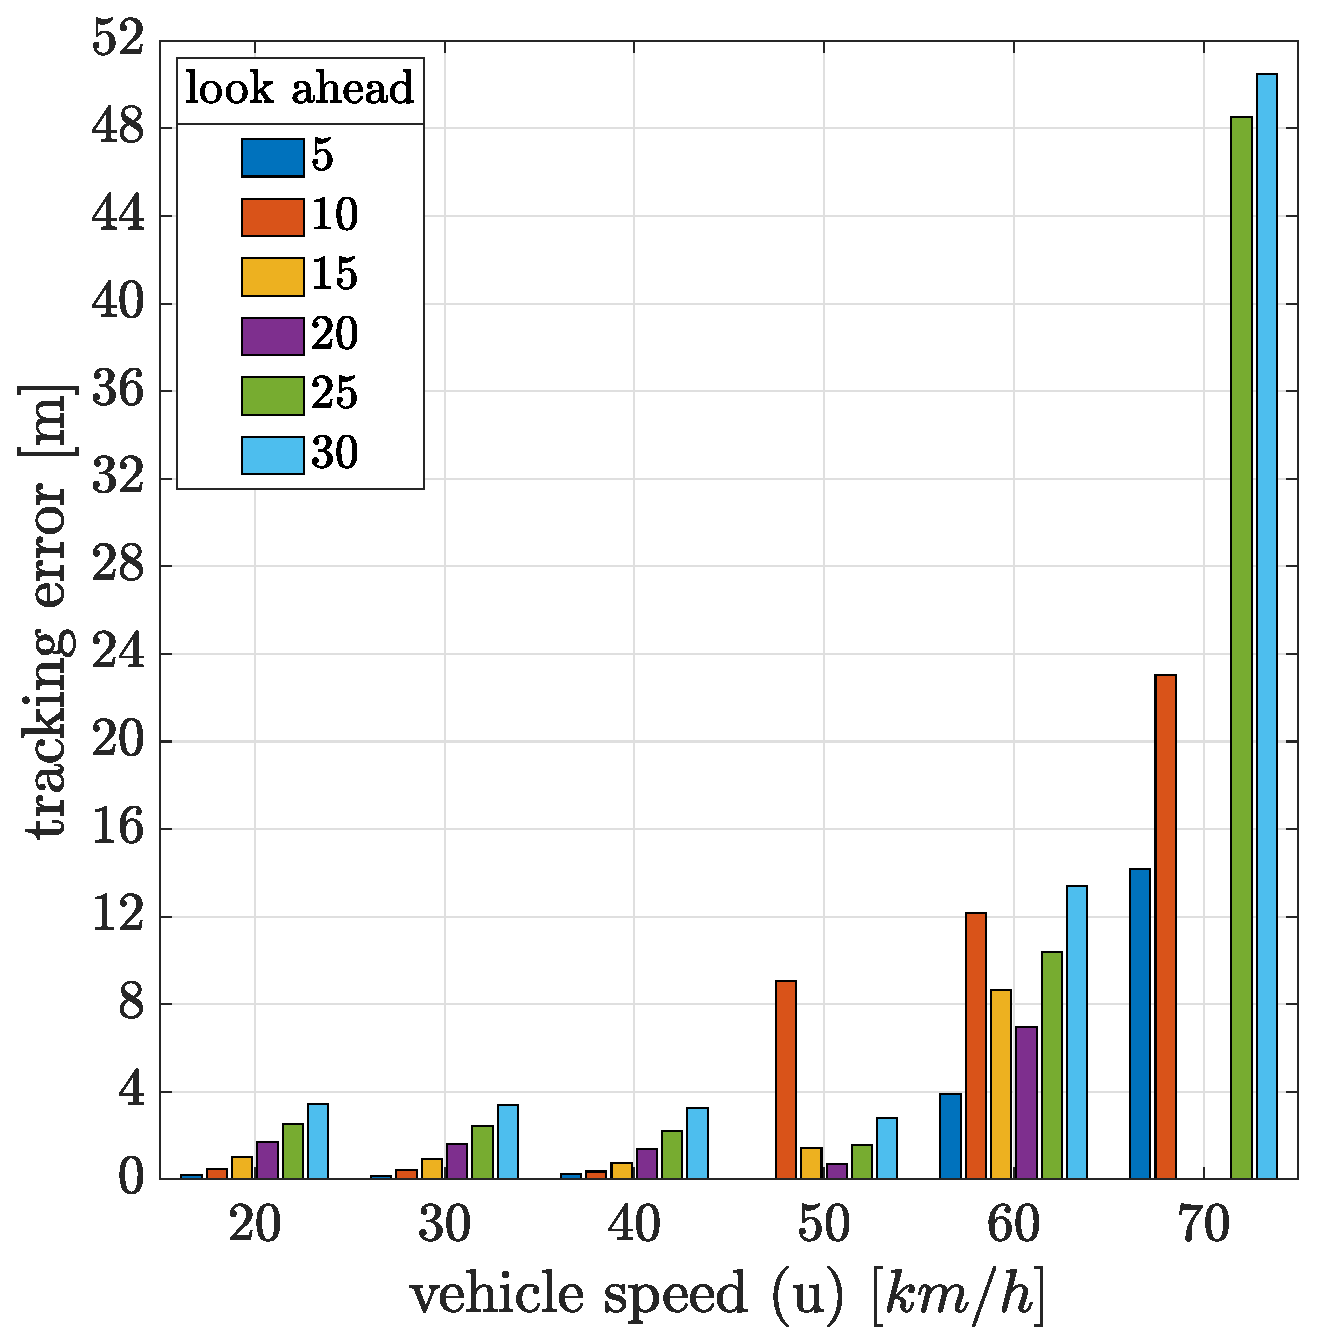
\includegraphics[width=0.6\linewidth]{ex6/q1/ex-61a.eps}
        \centering
        \caption{clothoid-based lateral controller at different $u$ and look ahead}
        \label{64d1}
        \end{figure}
      
The tests checked if the vehicle was able to arrive at a designated target point chosen to be at [60,10]. If the vehicle reaches this point within a threshold of 5 meters, the test is considered a success.

\begin{table}[ht]
    \centering
    \begin{tabular}{c | c | c| c | c | c | c }
      \textbf{$u$ [km/h]} & \textbf{LA = 5} & \textbf{LA = 10} & \textbf{LA = 15} & \textbf{LA = 20} & \textbf{LA = 25} & \textbf{LA = 30} \\ \hline
      20 &  \cellcolor{green!10}\num{0.212718999}	& \num{0.481794113}	& \num{1.025936442} &	\num{1.72651936}	& \num{2.534489657}	& \num{3.45986332}   \\\hline
      30 &  \cellcolor{green!10}\num{0.163715271} &	\num{0.431919243} &	\num{0.941254925} &	\num{1.632800857} &	\num{2.454559877} &	\num{3.408670041}\\\hline
      40 &  \cellcolor{green!10}\num{0.225603124} & \num{0.361992743}	& \num{0.728903508} &	\num{1.387858567} &	\num{2.228111216} &	\num{3.252073013}  \\\hline
      50 & \cellcolor{red!10}NA & \num{9.077008353} & \num{1.421928047} & \cellcolor{green!10}\num{0.718803621} &	\num{1.593478851} & \num{2.81030173} \\\hline
      60 &  \cellcolor{red!10}NA & \num{12.14781879} &	\num{8.667722795}	& \cellcolor{green!10}\num{6.971058339} & \num{10.36814129} & \num{13.42289353} \\\hline
      70 &  \num{14.15735028} & \num{23.03289356} & \cellcolor{red!10}NA & \cellcolor{red!10}NA & \num{48.50853335} & \cellcolor{green!10}\num{50.47894141}

    \end{tabular}
    \caption{Tracking error results [clothoid-based lateral controller]}
    \label{tab:6.1}
\end{table}

The red colored cells indicates the vehicle was not able to arrive at the designated target point. Green cells are the chosen look ahead values at each speed $u$.

It appears that the larger the look ahead value, the larger the tracking error as expected. Having a larger look ahead at 20 km/h could be beneficial if we are optimizing for traveled distance, and smoother turns [less jerk].

Figure \ref{61x20} shows the vehicle actual path at each look ahead value for 20 km/h tests. A larger look ahead optimized the vehicles path to take a shorter route and take better turns. However, this caused the tracking error to increase, because we are not following the reference trajectory anymore.

       \begin{figure}[ht]
        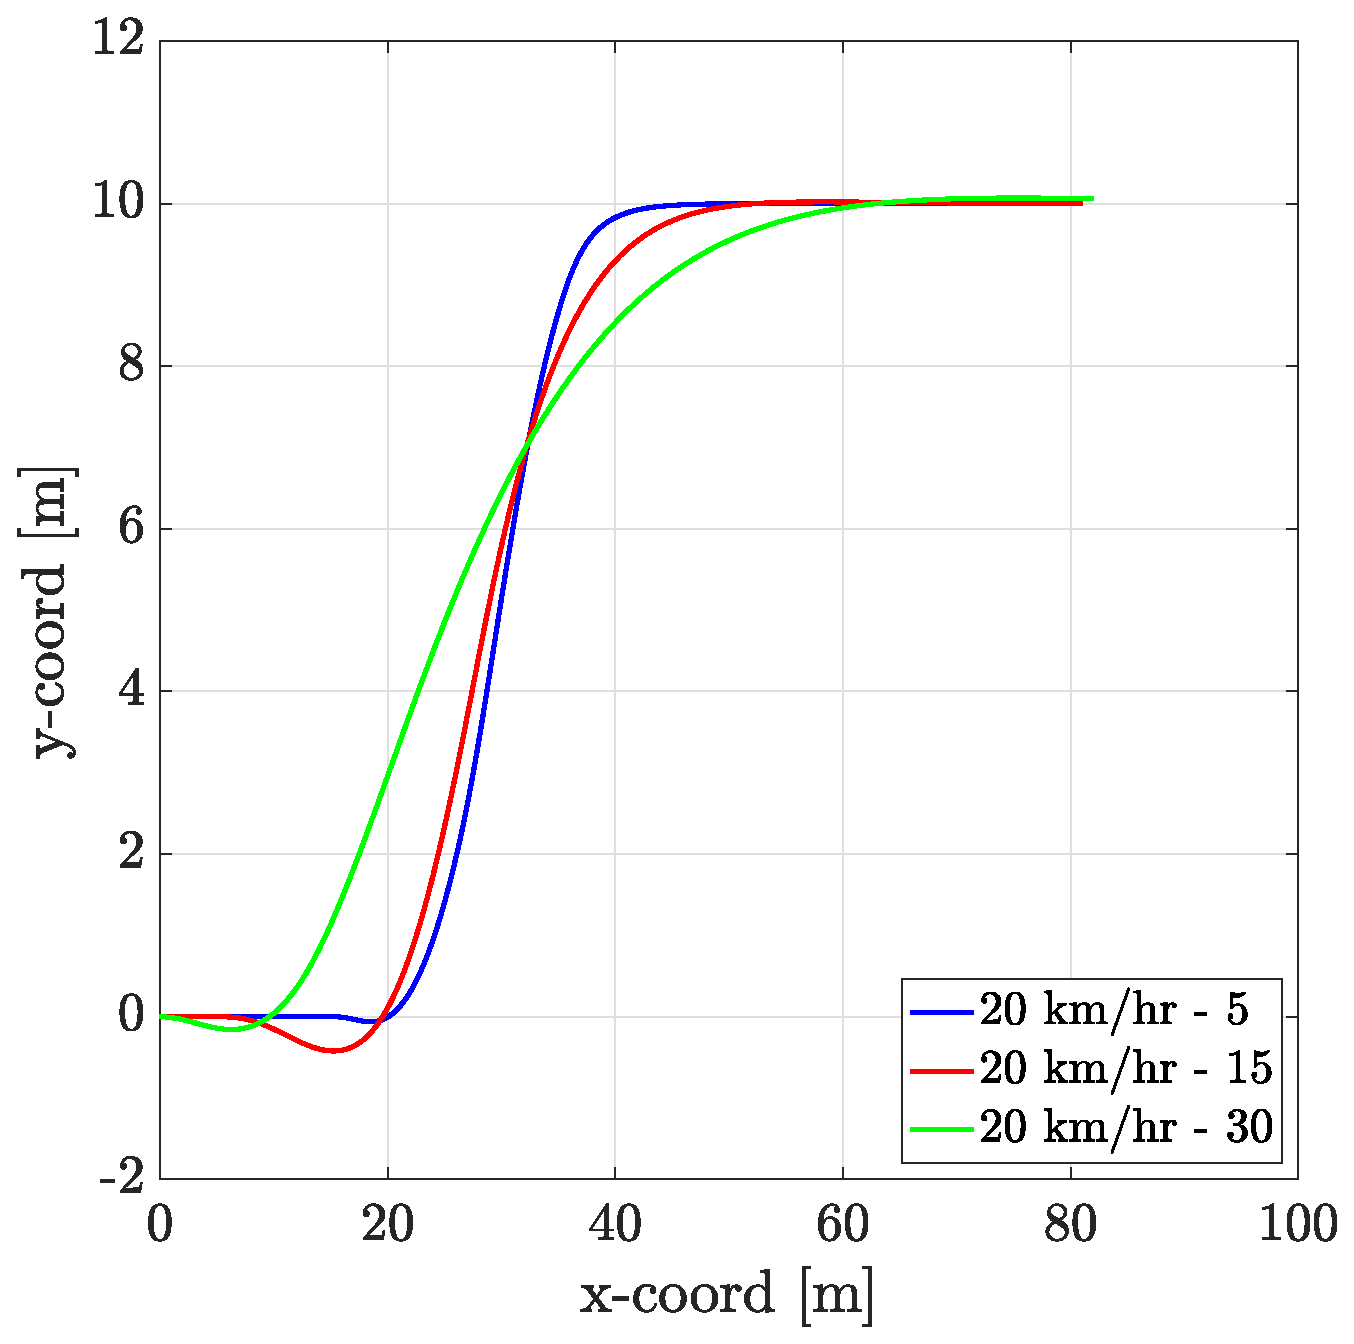
\includegraphics[width=0.6\linewidth]{ex6/q1/ex-61x20.eps}
        \centering
        \caption{Real vehicle path with different look ahead values [$u$ = 20km/h] }
        \label{61x20}
        \end{figure}

Up until 40 km/h, a lower look ahead value performed better for our metrics. With increasing $u$, the smaller look ahead values were simply not enough to control the vehicle properly. The controller needs to see far enough ahead to account for a curve earlier on. The faster the vehicle, the bigger the needed look ahead value. However, it seems that after 70 km/h, the vehicle can no longer become stable even with a look ahead as high as 250. 

Figure \ref{61x70} shows the vehicle paths at 70 km/h at different values for the look ahead. The higher values are more stable but still considered outside the capabilities of the vehicle.

No values of look ahead was enough to stabilize the vehicle with any speed higher than 70 km/h. This might be attributed to the $\kus$ values not accurate enough at these speeds. The handling curves during these speeds were not linear anymore and a linear approximation for them is not sufficient.

        \begin{figure}[ht]
        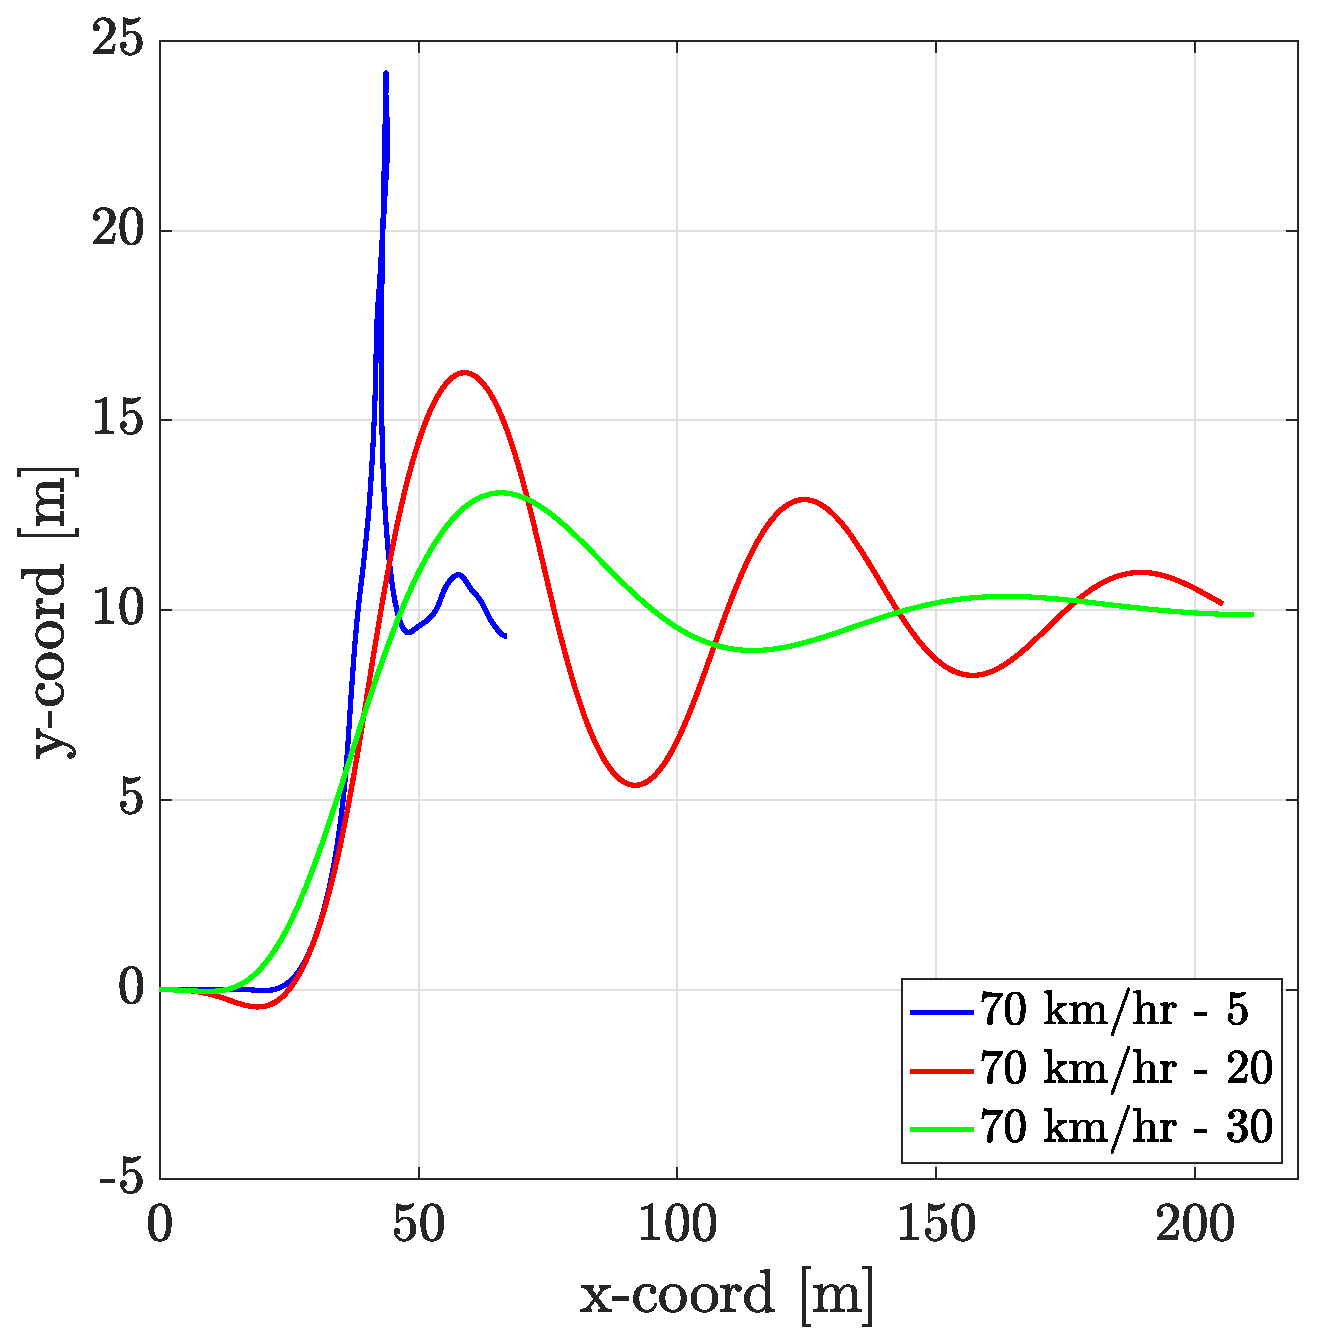
\includegraphics[width=0.6\linewidth]{ex6/q1/ex-61x70.eps}
        \centering
        \caption{Real vehicle path with different look ahead values[$u$ = 70km/h] }
        \label{61x70}
        \end{figure}

\textbf{Q. Implement the pure pursuit controller and optimize the look ahead distance}      
